\documentclass[11pt]{beamer}

\usepackage[utf8]{inputenc}
\usepackage[magyar]{babel}
\usepackage[T1]{fontenc}
\usepackage{lmodern}
\usepackage{zi4}
\usepackage{multirow}
\usepackage{listings}
\usepackage{ragged2e} % For \justifying command
\usepackage{color}

\usetheme{Warsaw}

\renewcommand\UrlFont{\ttfamily\footnotesize}

% no navigation symbols
\setbeamertemplate{navigation symbols}{} 

% frame numbers
\expandafter\def\expandafter\insertshorttitle\expandafter{%
  \insertshorttitle\hfill%
  \insertframenumber\,/\,\inserttotalframenumber}

\author{Nagy András}
\title{Komponens-alapú UML modellek fordításának vizsgálata}
\date{2019. január}

\begin{document}

\begin{frame}
\titlepage
\end{frame}

\begin{frame}[fragile]
	\frametitle{Problémakör háttere}
	
	\begin{itemize}
		\item \textit{txtUML} keretrendszerben írjuk le a komponens-alapú modellt, Java-szerű nyelven, mely végrehajtható.
		\item Lefordítható egy szabványos UML2 modellre.
		\item A cél a kompozit struktúrák és akciók megfelelő UML2-es szabványának megtalálása, melyből hatékony C++ kódot szeretnénk generálni.
	\end{itemize}
	
\end{frame}


\begin{frame}[fragile]
	\frametitle{Példa egy konkrét kompozit struktúrára}	
	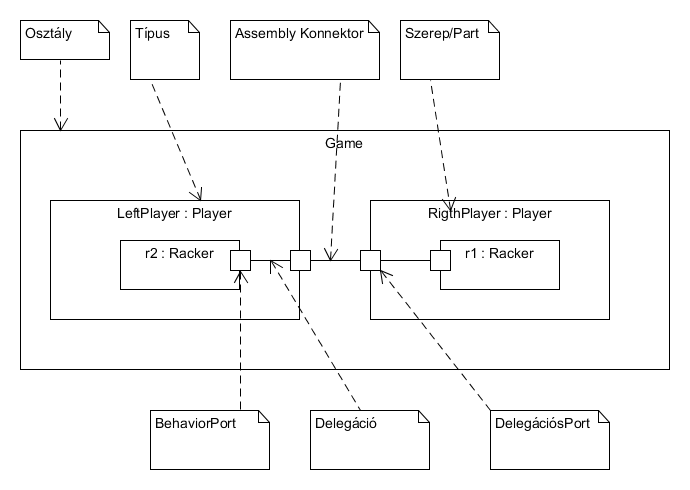
\includegraphics[scale=0.4]{vedes_demo.png}	
	
\end{frame}

\begin{frame}[fragile]	
	\frametitle{Értelmezési és reprezentációs problémák}	
	\begin{itemize}
	\item Port típusának reprezentálása, elvárt és szolgáltatott interfészek kifejezése.
	\item Két port összekapcsolása futási időben.
	\item Porta való üzenetküldés.
	\item Mi a szabványos modell végrehajtási szemantikája?
	\begin{itemize}
		\item UML2 szabvány.
		\item \textit{FUML} egy részhalmazához ad precíz szemantikát.
		\item \textit{PSCS} szabvány a kompozitokra próbálja kiegészíteni.
	\end{itemize}
	\end{itemize}
	
\end{frame}

\begin{frame}

	\frametitle{Példa: Konnektor, portok összekötése UML-ben}
	\begin{block}{UML specifikáció szerint}
	\textit{A Connector specifies links (see 11.5 Associations) between two or more instances playing owned or inherited roles within a StructuredClassifier." "A CreateLinkAction is a LinkAction for creating links."}
	\end{block}
	\begin{itemize}
	\item A \textit{Connector} értelemszerű (de mi az a \textit{type} referencia?)
	\item A problémás a \textit{connect} művelet
		\begin{itemize}
		\item Nincs \textit{connect} akció UML-ben
		\item \textit{DefaultConstructionStrategy}  (de az a szerkezet nem mindig egyértelmű..)
		\item A \textit{CreateLinkAction} segítségével összeköthetünk két portot a konnektor típusa mentén (Itt jön be a \textit{type} referencia, mely egy asszociációnak felel, ezt még ki kell generálni.).
		\end{itemize}
	\end{itemize}
\end{frame}


\begin{frame}[fragile]	
	\frametitle{C++-ra való fordítása}	
	\begin{itemize}
	\item Sok alternatíva (típusbiztonság, adatreprezentációs különbségek, stb.)
	\item Különböző elvárások a generált kóddal szemben (hatékonyság, olvashatóság, külső kóddal történő biztonságos illesztés, stb.)
	\item Ez a futási idejű könyvtár kialakításából és kódgenerálásból áll  az UML szemantika alapján.
	\item Ezeket a szempontokat figyelembe véve a munka elemzi az egyes kompozit elemek  kódgenerálási lehetőségeit.
	\end{itemize}
	
\end{frame}

\begin{frame}
	\frametitle{Üzenetáram eleje}
	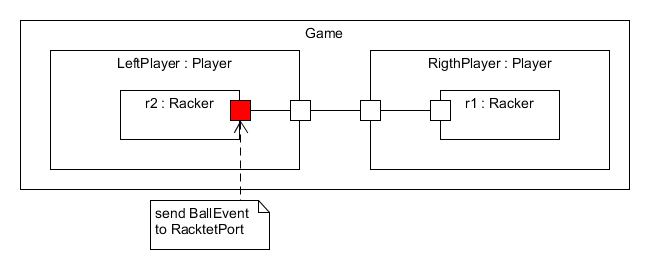
\includegraphics[scale=0.5]{vedes_demo_send.png}
	
	Kérdések: Hogyan alakítsuk ki a port osztályt C++-ban, hogyan küldünk rá üzenetet?
	
\end{frame}

\begin{frame}
	\frametitle{Üzenet továbbítása a szülő komponens felé - Delegáció}
	\begin{center}
	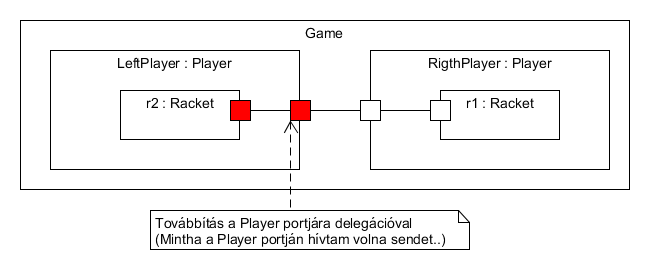
\includegraphics[scale=0.5]{vedes_demo_connect.png}
	\end{center}
	
	Problémák: Üzenet továbbítása szülő felé delegációs kapcsolat mentén.

\end{frame}


\begin{frame}
	\frametitle{Üzenet átadása testvér komponensek - Assembly}
	\begin{center}
	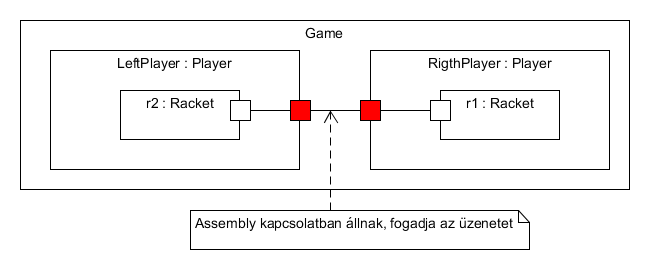
\includegraphics[scale=0.5]{vedes_demo_assconnect.png}
	\end{center}
	Problémák: Más a \textit{send} viselkedése, mint delegáció esetén, a port elvárt interfészének kell megfelelni. 
		
\end{frame}


\begin{frame}
	\frametitle{Üzenet továbbítása a gyerek komponensek}
	\begin{center}
	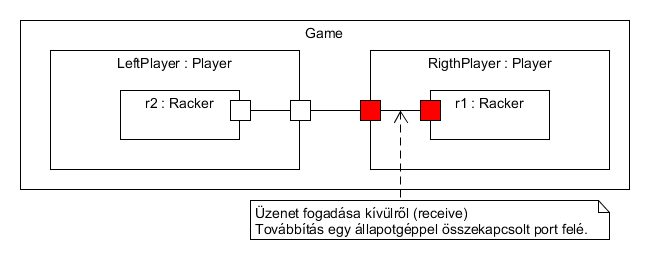
\includegraphics[scale=0.5]{vedes_demo_recived.png}
	\end{center}
	Delegációs kapcsolat másik iránya, a gyerek komponense felé továbbítom az üzenetet.
\end{frame}


\begin{frame}
	\frametitle{Gyerek felé továbbítás delegáció esetén}
	\begin{center}
	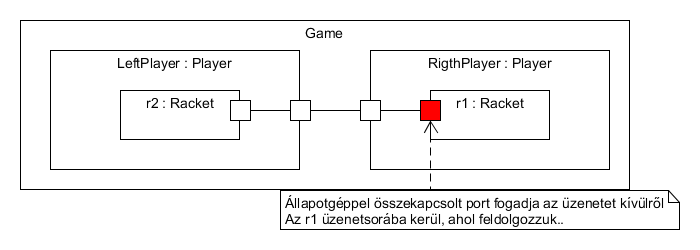
\includegraphics[scale=0.5]{vedes_demo_class_recived.png}
	\end{center}
	A gyerek komponens fogadó portja másképp kell, hogy viselkedjen, mint a szülőé, mivel állapotgéppel összekapcsolt port.
\end{frame}

\begin{frame}
	\frametitle{Portról jött üzenet feldolgozás}
	\begin{center}
	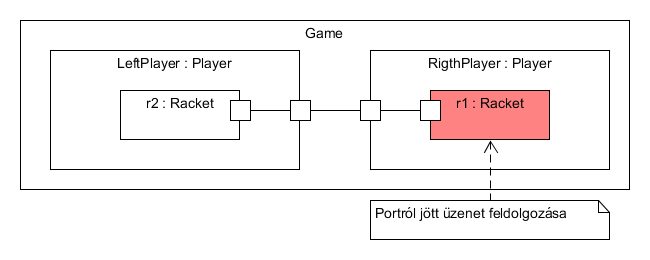
\includegraphics[scale=0.5]{vedes_demo_recived_proc.png}
	\end{center}
		Az üzenet az üzenetsorba kerül, fel kell dolgoznunk. Honnan tudjuk, melyik portról jött, átmenetetek kiterjesztése, hogy portról jött üzeneteteket is kezeljen.
\end{frame}

\begin{frame}
	\frametitle{Elemezett kódgenerálási stratégiák száma}
	
	\begin{center}
	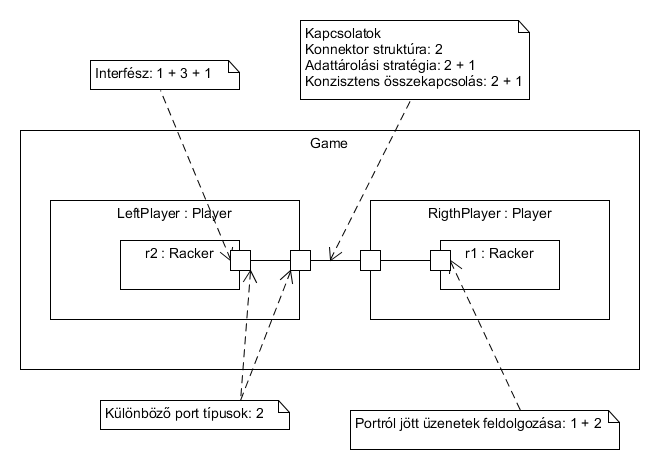
\includegraphics[scale=0.45]{vedes_demo_count.png}
	\end{center}
\end{frame}


\begin{frame}[fragile]
	\frametitle{Példa: Interfész kódgenerálási stratégiák}
	Nincs interfész, a forráskód validációja kiszűri a nem típusbiztos üzenetküldéseket. \\
	Előnyök:
	\begin{itemize}
		\item Triviális, nem kell dolgozni érte.
		\item Hatékony.
	\end{itemize}
	Hátrányok:
	\begin{itemize}
		\item Külső kóddal való illesztés nem biztonságos.
		\item Az interfész általánosabb fogalom, nem csak portok esetén akarom hsználni.
	\end{itemize}
	
		\begin{block}{Kódja}
	\begin{lstlisting}[basicstyle=\small])
class Port {
	...
	void send(GeneralEvent e);
	...
};
	\end{lstlisting}
	\end{block}
\end{frame}

\begin{frame}[fragile]
	\frametitle{Példa: Interfész kódgenerálási stratégiák - Van interfész}
	
	A fogadó szignálokat csoportosítsuk az interfészből történő leszármazással, a portnak legyen \textit{send} művelete, ami interfész leszármazottakat vár.
	Hátrányok:
	\begin{itemize}
	\item Nem elég általános megoldás.
	\item Interfészt nem csak portok, hanem bármilyen szereplők használhatnak, de ezzel csak portokra korlátoznánk a megoldást.
	\end{itemize}
	
		\begin{block}{Interfész kód}
	\begin{lstlisting}[basicstyle=\small])
class BallIfc {};
class Ball : public BallIfc {};

template<Ifc>
class Port { void send(Ifc& e); };

Port<BallIfc>
	\end{lstlisting}
	\end{block}

\end{frame}

\begin{frame}[fragile]
	\frametitle{Példa: Interfész kódgenerálási stratégiák}
	
	Az interfész legyen általános osztály annyi darab művelettel, ahány fogadó végpontja van. A port osztály valósítsa meg az interfészt, 
	Hátrányok:
	\begin{itemize}
	\item Jelentősen megnő a generált kód mérete.
	\item Funkcionálisan az összes művelet ugyanazt csinálja (így sablon metaprogramozással egyszerűsíthető..).
	\end{itemize}
	
	\begin{block}{Interfész kód}
	\begin{lstlisting}[basicstyle=\small])
class BallIfc {
public:
virtual void send(Ball& e) { sendAny(e)}; 
};

template<Ifc>
class Port : public Ifc {  };
	\end{lstlisting}
	\end{block}

\end{frame}

\begin{frame}[fragile]
	\frametitle{Példa: Interfész kódgenerálási stratégiák}
	
	Az interfészt bontsuk két részre, hogy a belső üzenetküldést, és a kívülről jött üzenetfogadást is ki tudja fejezni. 
	
	\begin{block}{Interfész kód}
	\begin{lstlisting}[basicstyle=\small])
class BallIfc {
class RequiredPart {
virtual void send(Ball& e) { sendAny(e)}; };
class ProvidedPart {
virtual void receive(Ball& e) { receiveAny(e)}; 
};
};
template<Provided, Required>
class Port :
 public Provided::ProvidedPart, 
 public Required::RequiredPart { 

};
	\end{lstlisting}
	\end{block}

\end{frame}

\begin{frame}
	\frametitle{A kertrendszer kompozíciós elemek támogatásának előnyei}
	
	\begin{itemize}
	\item Komponens modellezés támogatása (környezetfüggetlenség, újrafelhasználhatóság, stb.). 
	\item {txtUML} -> {FMU} exportálást hatékonyabban lehet megoldani. 
	\item Oktatási célok.
	\end{itemize}

\end{frame}

\begin{frame}
	\frametitle{Összefoglalás, eredmények}
	\begin{itemize}
	\item Az UML kompozit szabvány alapos értelmezése.
	\item Helyes reprezentáció használata.
	\item C++ kódgenerálási stratégiák elemezése, implementációval validálás.
	\item Szabványos modell generálása txtUML modell alapján, egy stratégia implementációja.
	\item \textit{txtUML} támogatja komponens-alapú modellezést, felhasználása..
	\end{itemize}
\end{frame}

\begin{frame}
	\frametitle{Komponens-alapú UML modellek fordításának vizsgálata}
	\begin{center}
		\Large{Köszönöm a figyelmet!}
	\end{center}
\end{frame}

\end{document}
